\documentclass[12pt]{article}
\usepackage{comment}
\usepackage[utf8]{inputenc}
\usepackage{xspace}
\usepackage{gastex}
\usepackage{amsmath}
\usepackage{amssymb}
\usepackage{wrapfig}
\usepackage{tikz}
\usepackage{float}
\usepackage{pgfplots}
\usepackage{booktabs} % For \toprule, \midrule and \bottomrule
\usepackage{pgfplotstable} % Generates table from .csvi
\usepackage{csquotes}
\usepackage{graphicx}
\usepackage{amsmath}
\usepackage{multicol}
\usepackage{tgtermes} % times font
\usepackage[shortlabels]{enumitem}
\usepackage{parskip}

\pagestyle{empty}
\textwidth      165mm
\textheight     252mm
\topmargin      -18mm
\oddsidemargin  -2mm
\evensidemargin -2mm
% \renewcommand{\baselinestretch}{0.96}
\newcommand{\impl}{\mathbin{\Rightarrow}}
\newcommand{\biim}{\mathbin{\Leftrightarrow}}
\newcommand{\id}[1]{\mbox{\textit{#1}}}
\newcommand{\tuple}[1]{\langle #1 \rangle}
\newcommand{\ma}{\mathsf{a}}
\newcommand{\mb}{\mathsf{b}}
\newcommand{\mc}{\mathsf{c}}
\newcommand{\md}{\mathsf{d}}
\newcommand{\nat}{\mathbb{N}}
\newcommand{\intg}{\mathbb{Z}}

\newcounter{question}
\newcommand{\question}[1]{
    \stepcounter{question}
    \thequestion. #1 \hfill
}

\newcommand{\revision}[1]{
    \stepcounter{question}
    \thequestion. #1* \hfill
}



\begin{document}
\topskip0pt
\begin{center}
    {\sc The University of Melbourne
        \\
        School of Computing and Information Systems
        \\
    COMP90020 Distributed Algorithms}
    \bigskip \\
    {\Large\bf Tutorial Week 9: Transactions and Concurrency Control}
    \bigskip \\
\end{center}

\section*{Notes}

\section*{Exercises}

\setcounter{question}{41}

% Serial Equivalence
% Conflicting Operation
% Pessimistic concurrency control: two phase locking, read locking, read-write locks
% Optimistic concurreny control: timestamp ordering, kung robinson
% nested transactions
\question{A server manages the objects $a_1, a_2, ..., a_n$. The server provides two operations for its
clients:}

\begin{itemize}
    \item $read (i)$: returns the $v$ of $a_i$
    \item $write(i, v)$: assigns $v$ to $a_i$
\end{itemize}
The transactions T and U are defined as follows:

\begin{itemize}
    \item $T: x = read(j); y = read (i); write(j, 44); write(i, 33);$
    \item $U: x = read(k); write(i, 55); y = read (j); write(k, 66).$
\end{itemize}


\begin{enumerate}[(a)]
    \item Give serially equivalent interleavings of T and U that are strict
    \item Give serially equivalent interleavings of T and U that are not strict but \textbf{could not produce} cascading aborts
    \item Give serially equivalent interleavings of T and U that \textbf{could produce} cascading aborts
\end{enumerate}

\bigskip

\question{The transfer transactions of T and U are defined as:}

\begin{itemize}
    \item $T: a.withdraw(4); b.deposit(4);$
    \item $U: c.withdraw(3); b.deposit(3);$
\end{itemize}

Suppose that they are structured as a pair of nested transactions

\begin{itemize}
    \item $T_1: a.withdraw(4); T_2: b.deposit(4);$
    \item $U_1: c.withdraw(3); U_2: b.deposit(3);$
\end{itemize}

\begin{enumerate}[(a)]
    \item Compare the number of serially equivalent interleavings of $T_1,T_2,U_1,U_2$ with the number of serially equivalent interleavings of $T$ and $U$.
    \item Explain why the use of these nested transactions generally permits a larger number of serially equivalent interleavings than non-nested ones.
\end{enumerate}

\bigskip

\question{Consider the recovery aspects of the nested transactions defined in the exercise above, assume that a withdraw operation will abort if the account will be overdrawn and that in this case the parent will also abort. }

\begin{enumerate}[(a)]
    \item Describe serially equivalent interleavings of $T_1, T_2, U_1, U_2$ that are strict
    \item Describe serially equivalent interleavings of $T_1, T_2, U_1, U_2$ that are not strict
    \item To what extent does the criterion of strictness reduce the potential concurrency gain of nested transactions?
\end{enumerate}

\question{The transactions T and U are defined as follows:}

\begin{itemize}
    \item $T: x = read(i); write(j, 44);$
    \item $U: write(i,55); write(j, 66);$
\end{itemize}

Initial values $a_i = 10, a_j = 20$. Which of the following interleavings are serially equivalent, and which could occur with two-phase locking?

\begin{center}
    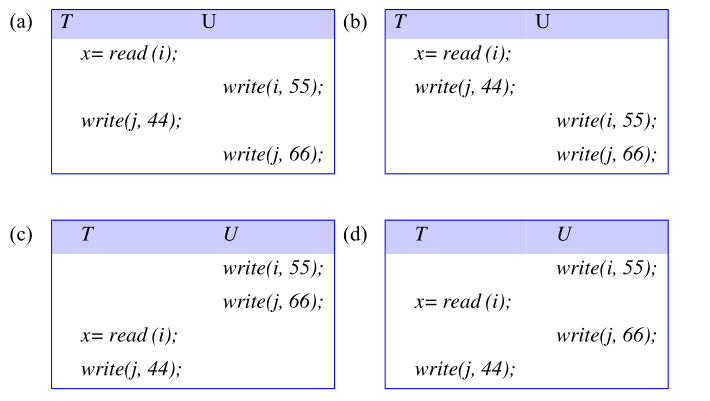
\includegraphics[width=0.75\textwidth]{2pc.png}
\end{center}

\bigskip

\question{Consider three concurrent transactions below}

\begin{center}
    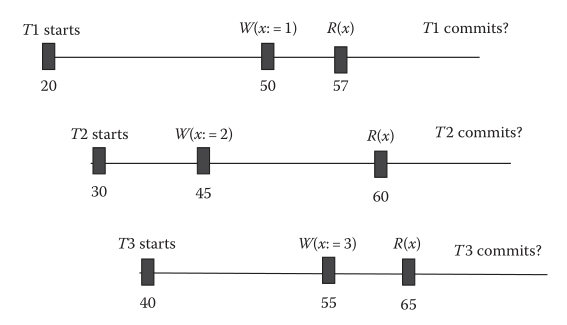
\includegraphics[width=0.75\textwidth]{ghosh.png}
\end{center}

Consider concurrency control by timestamp ordering. Which of these three concurrent transactions will commit?



\end{document}
